%% Preamble for this document
% Declare the document class with 12pt font
\documentclass[11pt]{article}
% Include the math package
\usepackage{amsmath}
% Include the math symbols package
\usepackage{amssymb}
% Use the geometry package to change the margins to 1"
\usepackage[margin=1in]{geometry}
% Include the graphicx package for inserting diagrams of the problem
\usepackage{graphicx}
% Enable using subFigures
\usepackage{subfig}

% Here's the document
\begin{document}

	% Create the title page
	\thispagestyle{empty}
	\pagenumbering{gobble}
	\title{MATH 189: Induction Proof}
	\author{Rob Peterson}
	\date{Fall 2017}
	\maketitle

	\newpage % Force a page break for the title page

	\pagenumbering{arabic} % Re-Start the page numbering

	%% Introduction section
	\section{Introduction}
		The problem under consideration in this document is a problem consisting of disks, an algorithm and a series of steps.  
		The problem is described as follows:\
		\begin{align*}
			1) &\text{ A stack of seven disks sits on a surface.}\\
			2) &\text{ One disk is added to the top of the existing stack(s),} \\
		    	    &\text{ and a set of disks is added to form a square perimeter around the existing stack(s).}\\
			3) &\text{ Step 2 is repeated ad Infinium.}
		\end{align*}	
		It is often easier to understand a problem if there are visual references available to the reader.  The author has provided these below:\
		\begin{figure}[h]
			\subfloat[Step 1]{
				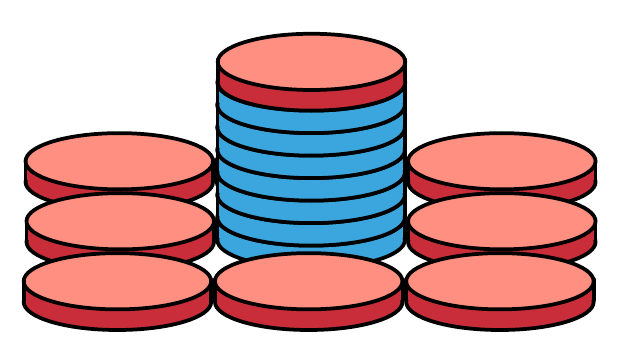
\includegraphics[width=.1\textwidth]{step1.png}
				\label{Step1_iso}
			}
			\subfloat[Step 2]{
				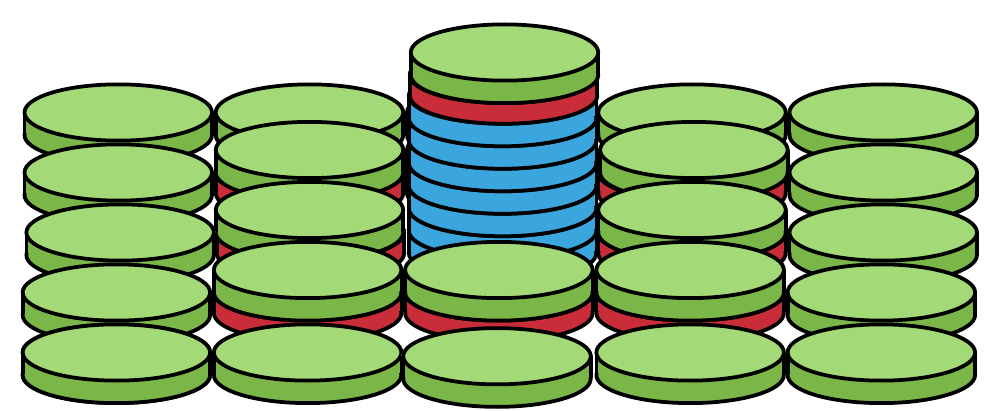
\includegraphics[width=.3\textwidth]{step2.png}
				\label{Step2_iso}
			}
			\subfloat[Step 3]{
				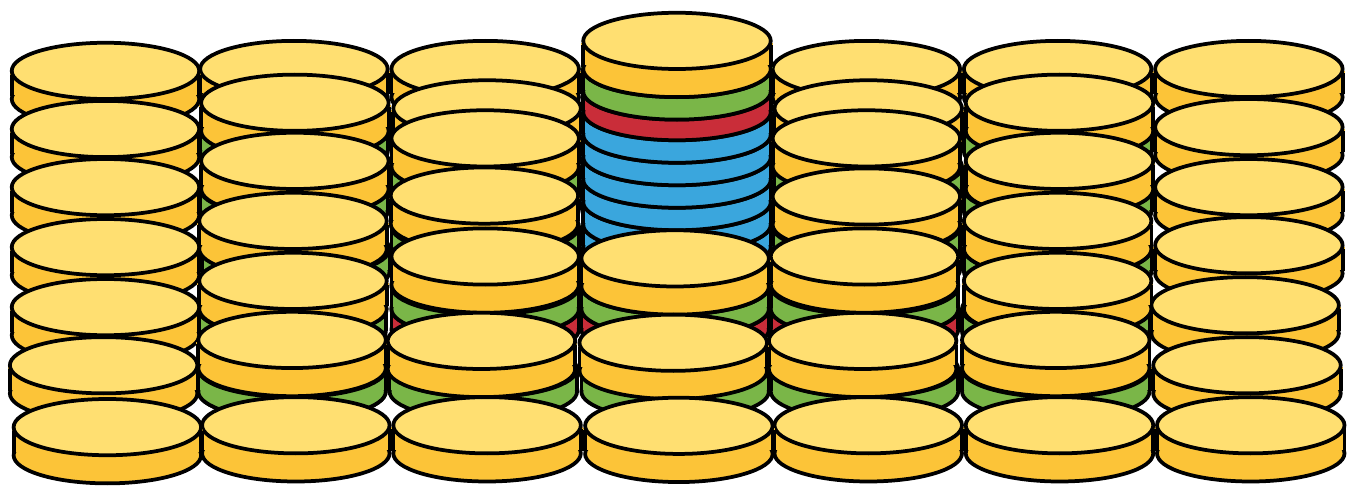
\includegraphics[width=.5\textwidth]{step3.png}
				\label{Step3_iso}
			}
			\\
			\begin{center}
			\subfloat[Step 4]{
				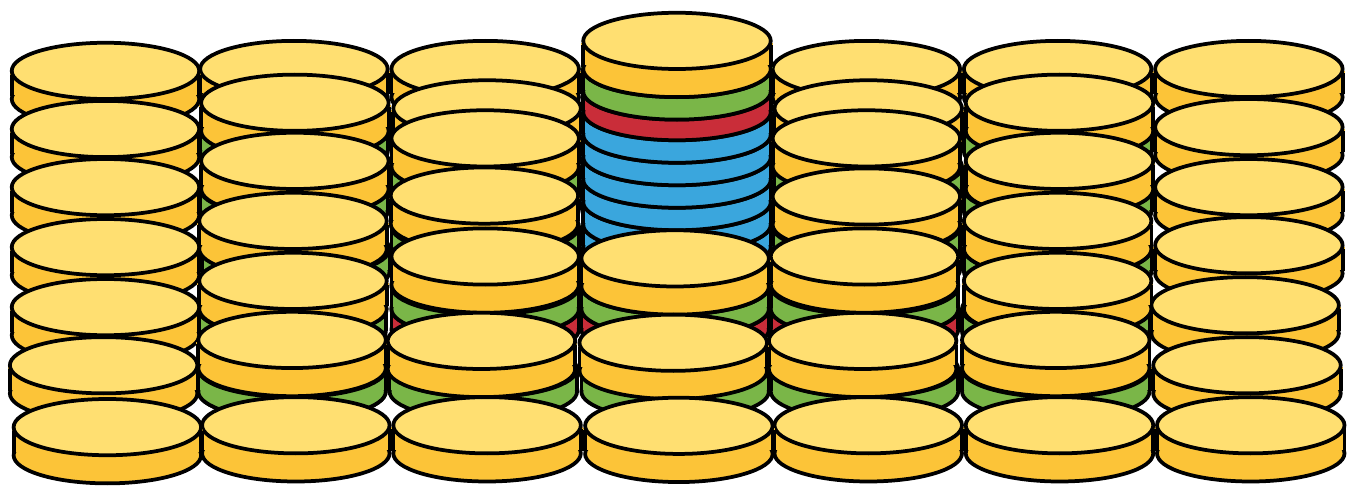
\includegraphics[width=.7\textwidth]{step4.png}
				\label{Step4_iso}
			}
			\end{center}
			\caption{Visualizations of the $1^{st}$ four problem steps.}
			\label{fig:disks_iso}
		\end{figure}
	\newpage
	\section{Recursive and closed form expressions}
		The ultimate goal is to use the principle of mathematical induction to prove the validity of a closed form expression 
		for describing the number of disks needed for any particular step of the problem statement.  This will involve four 
		steps; generating data, developing a recursive formula, developing a closed form expression, and finally using induction 
		to prove the close form to be correct.
	
	\subsection{Data}
		As shown in the isometric views of the problem seen in figure~\ref{fig:disks_iso}, the sides of the square of disks being put down are growing 
		at a rate of two disks per step.  This observation becomes very important in the development of this proof.  Since a top-down orthographic view will be easier to show
		the side length growth from step to step, the author has included them below:
		
		%% Top-down view of the figures (to see the square sizes better)
		\begin{figure}[h]
			\begin{center}
			\subfloat[Step 1]{
				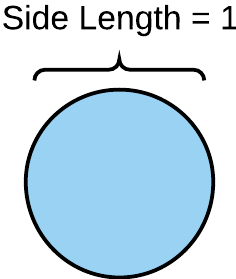
\includegraphics[width=.07\textwidth]{ortho1.png}
				\label{Step1_ortho}
			}
			\subfloat[Step 2]{
				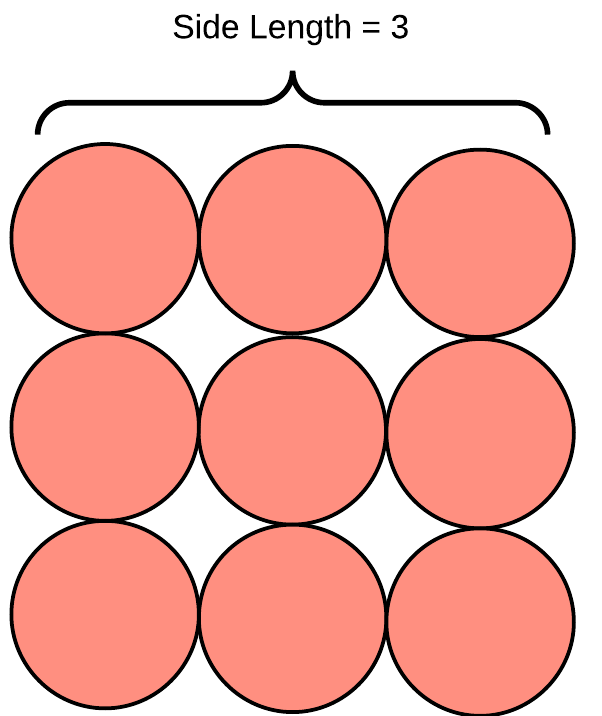
\includegraphics[width=.18\textwidth]{ortho2.png}
				\label{Step2_ortho}
			}
			\subfloat[Step 3]{
				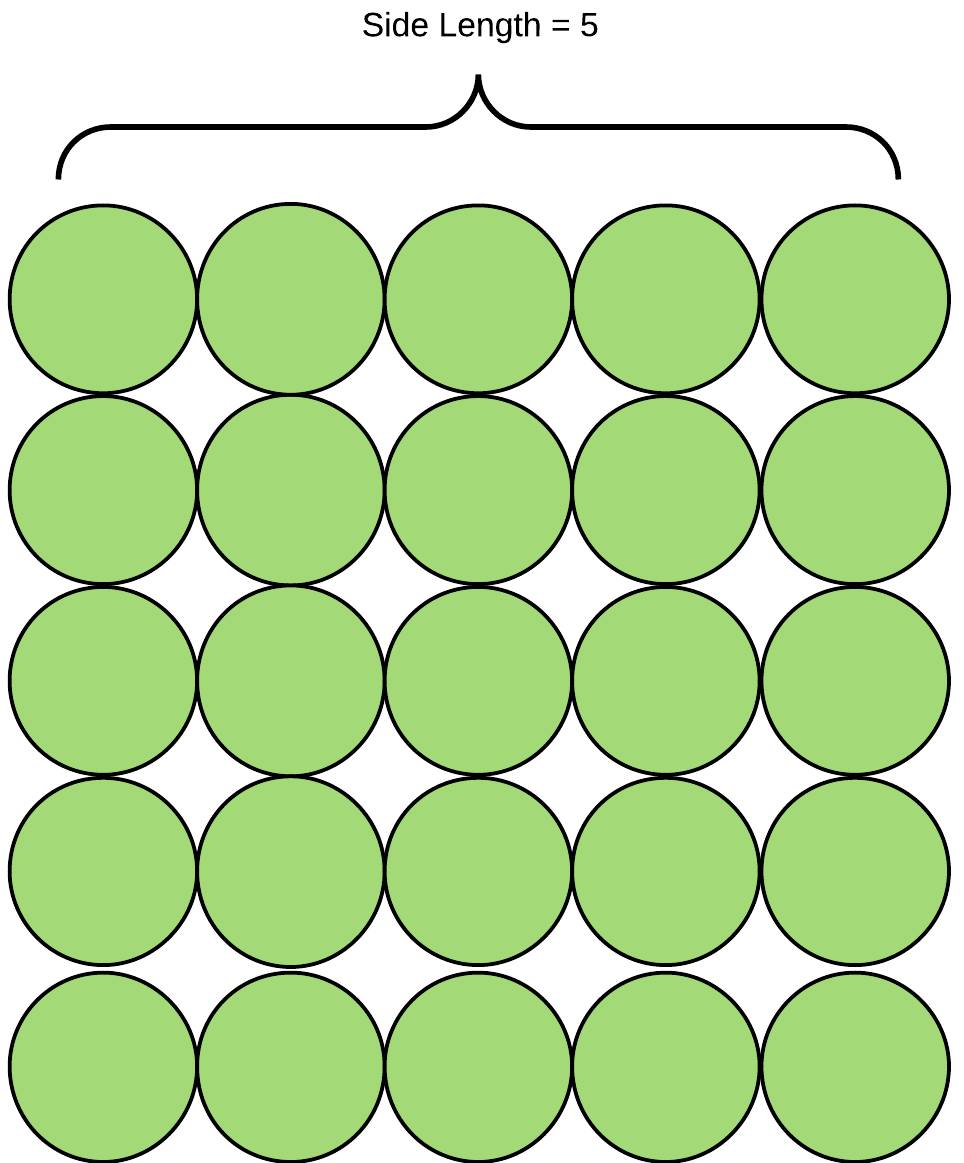
\includegraphics[width=.3\textwidth]{ortho3.png}
				\label{Step3_ortho}
			}
			\end{center}
			\begin{center}
			\subfloat[Step 4]{
				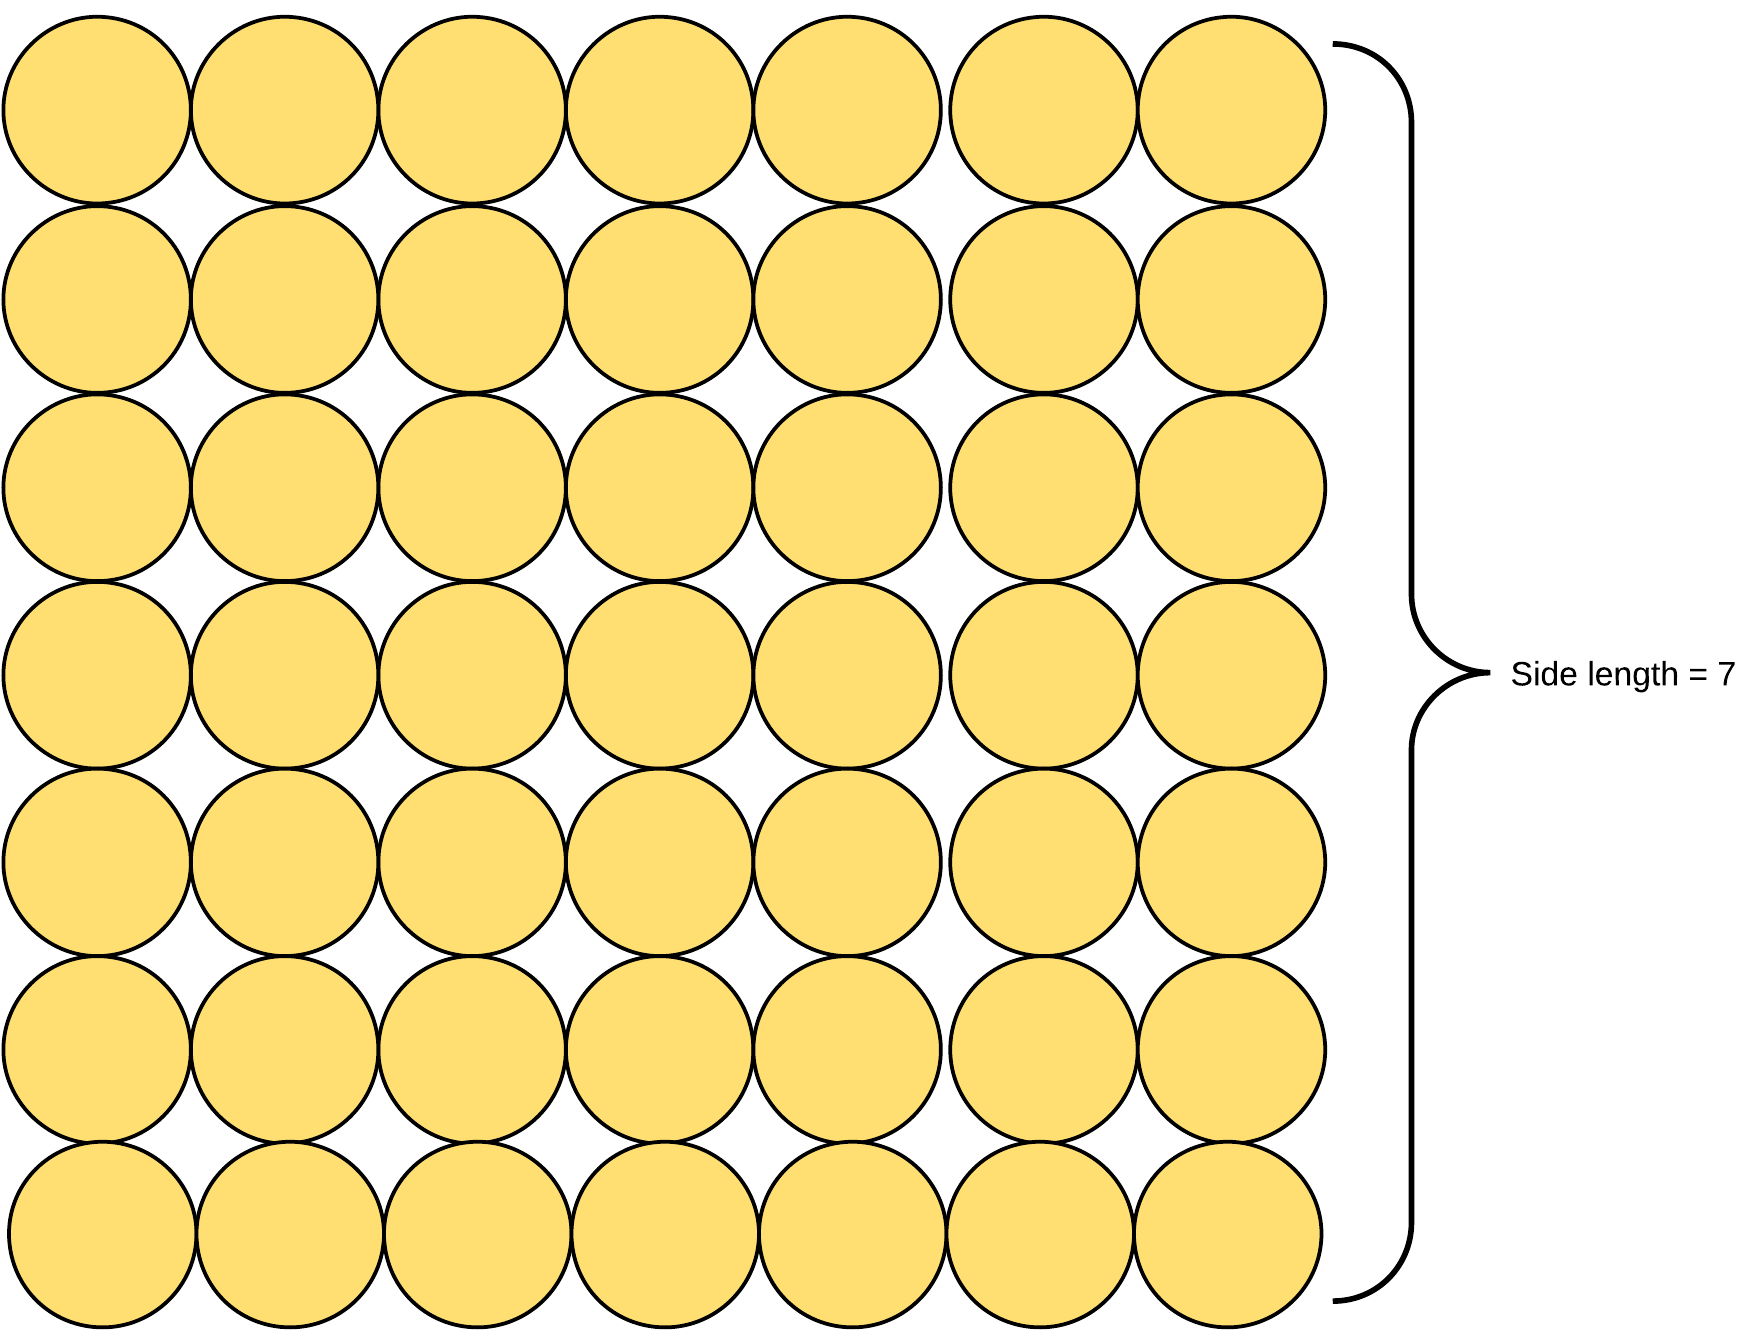
\includegraphics[width=.50\textwidth]{ortho4.png}
				\label{Step4_ortho}
			}
			\end{center}
			\caption{Top-down views of the $1^{st}$ four problem steps.}
			\label{fig:disks_ortho}
		\end{figure}

	\newpage

	As the reader can see from the top-down views on the previous page, the side length is an integer that starts at 1, and increases by 2 with each step.  
	For example, in \emph{Figure}~\ref{Step2_ortho}, we see a side length of 3, and in \emph{Figure}~\ref{Step3_ortho}, we see a side length of 5.  The second observation these
	orthographic views give us is the fact that the problem is creating squares of increasing size from step to step.\\
	
	If we define the length of a side of one of these squares as $l$, and the area of one of these squares as $a$, we can define the domain of $l$ and $a$ as a subset of the 
	natural numbers, or $l\in\mathbb{N}$ and $a\in\mathbb{N}$.  We can further restrict the domain of these variables using the observations stated above.  If we define $L$ to be the set
	that $l$ is a member of $(l\in L)$, and $A$ to the be set that $a$ is a member of $(a\in A)$, then we can express these two sets in set builder notation:

	\begin{align*}
		L&=\{x\in\mathbb{N}:x\text{ is odd}\}\\
		A&=\{y\in\mathbb{N}:y=x^2\}\\
	\end{align*}

	If we make another observation from \emph{Figure}~\ref{fig:disks_ortho}, we see that the left and right sides are always 2 disks smaller than the top and botton for steps $>1$.  
	This is mainly due to convention, since the top and bottom take up the full width of the squares.  We could have just as easily chosen the top and bottom to be 2 disks shorter than the 
 	sides.  The problem statement indicates that one new disk will be placed at every position on the perimeter, so we should derive an expression for the top/bottom and the left/right sides 
	of the perimeter.  Looking at some data may help us do that, the step number, top/botton length, and side length are tabulated below:

	\begin{center}
		\begin{tabular}{|c|c|c|}	\hline\hline
			\emph{step number} &
			\emph{top/bottom length} &
			\emph{left/right side length} \\ \hline
			1	&1	&1 \\
			2	&3	&1 \\
			3	&5	&3 \\
			4	&7	&5 \\ \hline \hline
		\end{tabular}
	\end{center}
	
	\subsection{Recursive Formula}

	We can see that the data shows the relationships between the step number and the side lengths.  The top/bottom side lengths are always one less than twice the step number, and the 
	left/right side lengths are always 2 less than the top/bottom side lengths.\
	If we define $n\in\mathbb{N}$ to be the step number, then we have the following for the top/bottom and left/right side lengths:
	\begin{center}
		\begin{align}
			l&=2n-1 \text{     (top/bottom side lengths)}\\
			2n-1-2&=2n-3 \text{     (left/right side lengths)}
		\end{align}
	\end{center}

	\newpage

	Another observation that we can make from the above table is that the left and right side lengths are always equal to the top/bottom
	side lengths from the previous step.  In the problem statement, we are adding one disk on top of all the existing stacks, so by definition, the previous step's contribution to the newly
	added disks will be the square of its top/bottom side lengths (the longest side).  This give us the following expression for the previous square's contribution to the new disks that are being
	added at each step:
	\begin{center}
		\begin{align}
			(2n-3)^2
		\end{align}
		\begin{align*}
			\text{(Previous steps' contribution to new layer of disks)}
		\end{align*}
	\end{center}

	Using equations 1,2 and 3, we can now build a recursive formula for determining the number of disks needed to complete each step.  If we define $n$ as done previously, and define 
	$D(n)$ to be the number of disks require to complete the $n^{th}$ step, we have the following:
	 	
	\begin{align}
		D(1)&=7 \quad \text{(Given in problem statement)}\\
		D(n)&= D(n-1)+(2n-3)^2+2(2n-1)+2(2n-3) \quad \text{(for $n>1$)}
	\end{align}

	The number of disks required for the first 6 steps in the problem statement will be useful for verifying work done so far, these numbers have been manually counted, and are
	tabulated here:

	\begin{center}
		\begin{tabular}{|c|c|c|}	\hline\hline
			\emph{step number } $(n)$ &
			\emph{disks needed} \\ \hline
			1	&7	\\
			2	&16	\\
			3	&41	\\
			4	&90	\\
			5	&171 	\\
			6	&292	\\ \hline \hline
		\end{tabular}
	\end{center}

	We can verify the recursive formula 5 by plugging in $n=2$ and $n=3$ to equation 5, and comparing the results to the table.

	\begin{align*}
		D(2)&= D(2-1)+(2(2)-3)^2+2(2(2)-1)+2(2(2)-3) \\
		&=7+(1)^2+2(3)+2(1)=7+1+6+2=16 \quad \checkmark \\
		D(3)&= D(3-1)+(2(3)-3)^2+2(2(3)-1)+2(2(3)-3) \\
		&=16+(3)^2+2(5)+2(3)=16+9+10+6=41 \quad \checkmark
	\end{align*}

	\newpage
	
	\subsection{Closed Form}

	We can use the data table that we have to develop a closed form expression for the number of disks required at a particular step.  One way of doing this is to perform a differencing
	technique.  

	\begin{align}
		D(k+1)&=D(k)+(2(k+1)-3)^2+2(2(k+1)-1)+2(2(k+1)-3)\\
		&=D(k)+(2k+2-3)^2+2(2k+2-1)+2(2k+2-3)\\
		&=D(k)+(2k-1)^2+2(2k+1)+2(2k-1)\\
		&=D(k)+(2k-1)^2+4k+2+4k-2\\
		&=D(k)+4k^2-4k+1+4k+2+4k-2\\
		&=D(k)+4k^2+4k+1		
	\end{align}
	\text{We've assumed that the closed form formula is valid for D(k)}
	\begin{align}
		D(k+1)&=[\frac{4}{3}k^3-\frac{1}{3}k+6]+4k^2+4k+1\\	
		&=\frac{4k^3-k+18}{3}+4k^2+4k+1\\
		&=\frac{4k^3-k+18+12k^2+12k+3}{3}\\
		&=\frac{4k^3+12k^2+11k+21}{3}\\
		&=\frac{4k^3+12k^2+(12k-1k)+(-1+18+4)}{3}\\
		&=\frac{[4k^3+12k^2+12k+4]+[-1k-1]+18)}{3}\\
		&=\frac{4[k^3+3k^2+3k+1]-[k+1]+18)}{3}\\
		&=\frac{4(k+1)^3-(k+1)+18)}{3}\\
		&=\frac{4(k+1)^3}{3}-\frac{(k+1)}{3}+6
	\end{align}
	By mathematial induction, the preceding has proven that the closed form formula expressed in equation 12 accurately describes how many 
	disks would be needed to complete any particular step in the problem statement.
\end{document}